\documentclass[12pt,a4paper]{scrartcl}
\usepackage[utf8]{inputenc}
\usepackage[english, russian]{babel}
\usepackage{indentfirst}
\usepackage{misccorr}
\usepackage[dvipdfmx]{graphicx}
\usepackage{amsmath}
\usepackage{multirow}
\usepackage{pgfplots}
\usepackage{parskip}
\usepackage[top=1cm, bottom=1cm, left=1cm, right=1cm]{geometry}
\pgfplotsset{compat=1.9}

\begin{document}
	\graphicspath{{pic/}, {~/Pictures/TeXImgs/}}
	
	\newcommand{\ms}{\mathstrut}
	\newcommand{\msp}{\hspace{0.5cm}}
	\newcommand{\al}{\alpha}
	\newcommand{\dg}{^\circ}
	\newcommand{\dif}{\mathrm{d}}
	\newcommand{\qd}[2]{^{\frac{#1}{#2}}}
	\newcommand{\qdm}[2]{^{-\frac{#1}{#2}}}
	\newcommand{\lm}[2]{\underset{#1 \rightarrow #2}{\lim}}
	\newcommand{\sfrac}[2]{\dfrac{\strut #1}{\strut #2}}
	\newcommand{\equal}[1]{\overset{(#1)}{=}}
	\newcommand{\linevdots}{\ \raisebox{-.08\height}{\vdots}\ }
	\newcommand{\linecvdots}{\ \raisebox{-.08\height}{\vdots}\hspace{-0.13cm}\raisebox{.15\height}{\cancel{\phantom{a}}\hspace{0.06cm}}}
	\newcommand{\combox}[1]{\ms \msp \msp \begin{minipage}{0.95\linewidth}
			#1
	\end{minipage}}
	
	\newtheorem{pr}{Задача}
	\newtheorem{ex}{Пример}
	\newtheorem{dfn}{Def}
	\newtheorem{theorem}{Th}
	
	\newenvironment{slv}{\ms \msp \textit{Решение:}}{}
	\newenvironment{proof}{\ms \msp \textit{Доказательство: }}{\hfill $\square$}
	
	\begin{titlepage}
		
		\vspace*{\fill}
		
		\begin{center}
			
\includegraphics[scale=0.8]{MIPT.png}
			\\[0.7cm]\Huge Московский Физико-Технический Институт\\(национальный исследовательский университет)
			\\[2cm]\LARGE Отчет по эксперименту
			\\[0.5cm]\noindent\rule{\textwidth}{1pt}
			\\\Huge\textbf{Петля гистерезиса\\(динамический метод)}
			\\[-0.5cm]\noindent\rule{\textwidth}{1pt}
		\end{center}
		
		\begin{flushleft}
			\textit{Работа №3.4.5; дата: 04.11.22}\hfill\textit{Семестр: 3}
		\end{flushleft}
		
		\vspace*{\fill}
		
		\begin{flushleft}
			Выполнил: \hspace{\fill} Группа:
			\\Кошелев Александр \hspace{\fill} Б05-105
		\end{flushleft}
	\end{titlepage}
	
	%Страница 2
	
	\begin{flushleft}
		\footnotesize{Петля гистерезиса (динамический метод)} \hspace{\fill} \footnotesize{2}
		\\[-0.3cm]\noindent\rule{\textwidth}{0.3pt}
	\end{flushleft}
	
	\section{Аннотация}
	
	\textbf{Цель работы: }
	
	Изучение петель гистерезиса различных ферромагнитных материалов в переменных полях.
	
	\textbf{Схема установки:}
	\begin{center}
		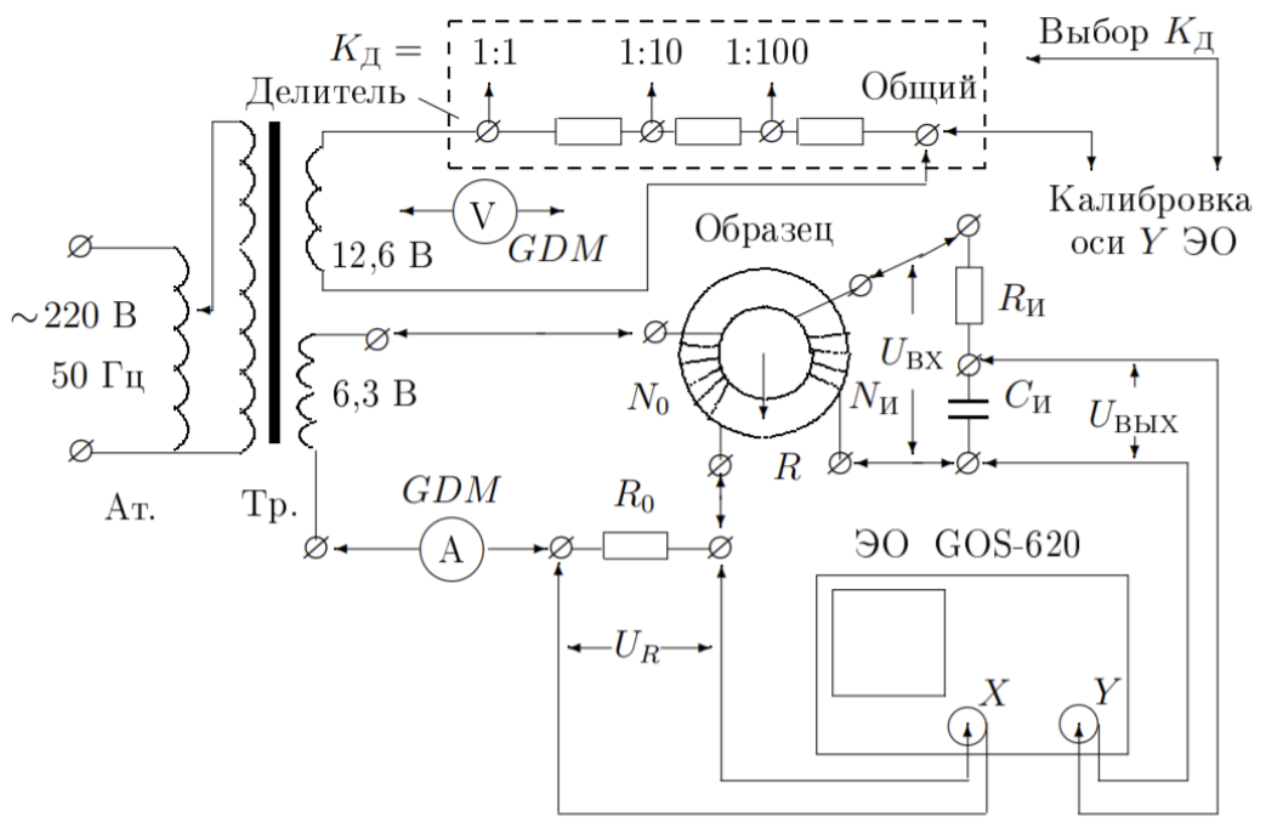
\includegraphics[scale=0.2]{PIC_1.png}
		\\\textbf{Рис. 1:} Схема установки
	\end{center}	
		
	Схема установки изображена на рисунке. Напряжение сети с помощью трансформаторного блока $T$, состоящего из 	регули­ровочного автотрансформатора и разделительного понижающего трансформатора, подаётся на 						намагничивающую обмотку $N_0$ исследуемого образца.
	
	В цепь намагничивающей катушки, на которую подаётся некоторое напряжение $U_0$, последовательно включено 		сопротивление $R_0$. Напряже­ние на $R_0$, равное $U_R = I_0 R_0$ , где $I_0$ -- ток в намагничивающей 			обмот­ке $N_0$, подаётся на канал $X$ осциллографа. Связь напряжённости $H$ в образце и тока $I_0$ 				рассчитывается по теореме о циркуляции. Действующее значение переменного тока в обмотке $N_0$ измеряется 		амперметром $A$.
	
	Для измерения магнитной индукции $B$ с измерительной обмотки $N_{\text{и}}$ на вход $RC$-цепочки подаётся 		напряжение $U_{\text{и}}$ ($U_{\text{вх}}$), пропорциональное производной $\dif B/\dif t$. С интегрирующей 		ёмкости $C_{\text{и}}$ снимается напряже­ние $U_{\textbf{и}}$ ($U_{\text{вых}}$), пропорциональное величине 		$B$, и подаётся на вход $Y$ осциллографа.

	Замкнутая кривая, возникающая на экране, воспроизводит в неко­тором масштабе (различном для осей $X$ и $Y$) 		петлю гистерезиса. Что­бы придать этой кривой количественный смысл, необходимо установить масштабы 				изображения, т. е. провести калибровку каналов $X$ и $Y$ осцил­лографа.

	\textbf{В работе используются:}
	
	Автотрансформатор, понижающий трансформатор, интегрирующая цепочка, амперметр, вольтметр, электронный 			осциллограф, делитель напряжения, тороидальные образцы с двумя обмотками.

	\section{Теоретические сведения}

	\paragraph{Петля гистерезиса} \hfill
	
	Основные характеристики
ферромагнетиков — их коэрцитивное поле $H_c$, магнитная проницаемость
$\mu$, рассеиваемая в виде тепла при перемагничивании мощность — зависят
от частоты перемагничивающего поля. В данной работе кривые гистерезиса ферромагнитных материалов изучаются в поле частоты $\nu_0 =$ 50 Гц
с помощью электронного осциллографа.

	\newpage

	%Страница 3

	\begin{flushleft}
		\footnotesize{Петля гистерезиса (динамический метод)} \hspace{\fill} \footnotesize{3}
		\\[-0.3cm]\noindent\rule{\textwidth}{0.3pt}
	\end{flushleft}	
		
	\begin{center}
		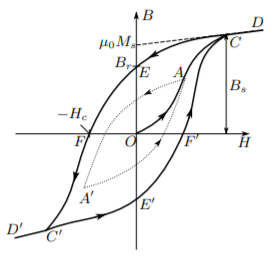
\includegraphics[scale=0.8]{PIC_2.png}
		\\\textbf{Рис. 2: } Петля гистерезиса ферромагнетика
	\end{center}
	
	Магнитная индукция $ B $ и напряжённость поля $ H $ в ферромагнитном материале неоднозначно связаны между собой: индукция зависит
не только от напряжённости, но и от предыстории образца. Связь между $ B $ и $ H $ типичного ферромагнетика иллюстрирует рис. 2.

Если к ферромагнитному образцу прикладывать переменное внешнее
магнитное поле, то его состояние на плоскости $ B-H $ будет изменяться
по замкнутой кривой — петле гистерезиса. Размер петли определяется
максимальным значением напряжённости $ H $ в цикле (например, петля $ AA' $,
обозначенная пунктиром на рис. 2). Если амплитуда напряжённости достаточно велика, то образец будет периодически достигать насыщения,
что на рисунке соответствует кривой $ CEFC'E'F'C $ (предельная петля
гистерезиса). Пересечение предельной петли с вертикальной осью соответствует остаточной индукции $B_r$, пересечение с горизонтальной осью
— коэрцитивному полю $H_c$. Крайние точки петель, соответствующие амплитудным значениям $ H $ (например, точка $ A $ на рис. 2), лежат на начальной кривой намагничивания ($ OAC $).
	
	\paragraph{Измерение магнитной индукции} \hfill
	
	Магнитную индукцию $ B $ удобно
определять с помощью ЭДС, возникающей при изменении магнитного
потока $ \Phi $ в катушке, намотанной на образец. Пусть катушка c $ N $ витками плотно охватывает образец сечением $ S $, и индукция $ B $ в образце
однородна. Тогда	

	$$|B|=\frac{1}{SN}\int\mathcal{E} dt$$
	
Для интегрирования в работе используется интегрирующая $ RC $-цепочка.	

	\begin{center}
		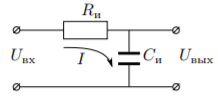
\includegraphics[scale=0.8]{PIC_3.png}
		\\\textbf{Рис. 3: } Интегрирующая ячейка
	\end{center}
	
	«Входное» напряжение от источника $U_{\text{вх}}(t)$ подаётся на последовательно соединённые резистор $R_\text{и}$ и конденсатор $C_\text{и}$. <<Выходное>>
напряжение $U_{\text{вых}}(t)$ снимается с конденсатора. Предположим, что сопротивление источника мало по сравнению с $R_\text{и}$; выходное сопротивление (сопротивление на входе осциллографа), напротив, велико: $R_{\text{вых}}$ $ \gg $ $R_\text{и}$ и, наконец, сопротивление $R_\text{и}$ достаточно велико, так что почти всё падение напряжения приходится на него, а $U_{\text{вых}}$ $\ll$ $U_{\text{вх}}$. В таком случае ток цепи равен I = ($U_{\text{вх}}$ - $U_{\text{вых}}$)/$R_\text{и}$ $\approx$ $U_{\text{вх}}$/$R_\text{и}$, и входное и выходное сопротивление связаны соотношением

	$$U_{\text{вых}} = \frac{q}{C_\text{и}} = \frac{1}{C_\text{и}}\int\limits_0^t Idt \approx \frac{1}{\tau_\text{и}} \int\limits_0^t U_{\text{вх}}dt$$
	
	\newpage
	
	%Страница 4
	
	\begin{flushleft}
		\footnotesize{Петля гистерезиса (динамический метод)} \hspace{\fill} \footnotesize{4}
		\\[-0.3cm]\noindent\rule{\textwidth}{0.3pt}
	\end{flushleft}	
	
где $\tau_\text{и}=R_\text{и}C_\text{и}$ - постоянная времени $ RC $ - цепочки. Для индукции поля из получаем

$$|B|=\frac{1}{SN}\int U_{\text{вх}} dt=\frac{\tau_\text{и}}{SN}U_{\text{вых}}.
$$

Уточним критерий применимости. Пусть на вход интегрирующей ячейки подан синусоидальный сигнал с частотой $\omega_0$. Тогда, пользуясь методом комплексных амплитуд, нетрудно найти отношение амплитуд входного и выходного напряжений: 
	
$$\frac{U_{\text{вых}}}{U_{\text{вх}}}=\frac{1/\omega_0C}{\sqrt{R^2+1/(\omega_0C)^2}}$$
	
Тогда неравенство $U_{\text{вых}} \ll U_{\text{вх}}$ реализуется, если 

$$\tau \equiv RC\gg \frac{1}{\omega_0}$$	
	
(импеданс конденсатора мал по сравнению сопротивлением резистора).
В таком случае для синусоидального сигнала имеем

$$\frac{U_{\text{вых}}}{U_{\text{вх}}}\approx\frac{1}{\omega_0\tau}$$

В общем случае, если $\omega_0$ — частота самой низкой гармоники в спектре
произвольного входного сигнала, то при $\omega_0\tau \gg 1$ неравенство $U_{\text{вых}} \ll U_{\text{вх}}$ выполняется на любой частоте $\omega > \omega_0$.	
	
\section{Ход работы}
\paragraph{Измерение петель гистерезиса} \hfill

Соберем схему согласно схеме установки. Подберем ток питания в намагничивающей обмотке с помощью автотрансформатора и коэффициенты усиления ЭО таким образом, чтобы предельная петля гистерезиса занимала большую часть экрана. Приведем характерные значения катушек разных материалов в таблице.	

\begin{center}
	\begin{tabular}{|c|c|c|c|c|}
		\hline
		Материал     & $N_0$ & $N_\text{и}$ & $S^2$, см$^2$ & $2\pi R$, см \\ \hline
		Феррит       & 40    & 400                              & 3,0           & 25,0         \\ \hline
		Пермаллой    & 20    & 300                              & 0,8           & 13,3         \\ \hline
		Крем. железо & 25    & 250                              & 2,0           & 11,0         \\ \hline
	\end{tabular}
	\\\textbf{Табл. 1:} Характеристики катушек
\end{center}
	
Для каждого образца получим передельные петли гистерезиса, по коэффициентам усиления ЭО $K_x$ и $K_y$ рассчитаем масштабы, определим двойные амплитуды коэрцетивной силы $ [2x(c)] $ и индукции насыщения $ [2y(s)] $. Масштабы по осям $ X $ и $ Y $ рассчитаем по формулам 
$H=IN_0/(2\pi R),\ где\ I=K_x/R_0;\ B=R_\text{и}C_\text{и}U_{\text{вых}}/(SN_\text{и}),$ где $U_{\text{вых}}=K_y$. Результаты измерений и вычислений занесём в таблицы.

\begin{center}
	\begin{tabular}{|c|c|c|c|c|}
		\hline
		Материал     & $[2x(c)]$, дел & $[2y(s)]$, дел & $K_x$, мВ/дел & $K_y$, мВ/дел \\ \hline
		Феррит       & 1,0            & 4,8            & 20            & 20            \\ \hline
		Пермаллой    & 3,6            & 3,6            & 20            & 50            \\ \hline
		Крем. железо & 1,2            & 4,4            & 100           & 50            \\ \hline
	\end{tabular}
	\\\textbf{Табл. 2:} Масштабы по осям
\end{center}	
	
	\newpage
	
	%Страница 5
	
	\begin{flushleft}
		\footnotesize{Петля гистерезиса (динамический метод)} \hspace{\fill} \footnotesize{5}
		\\[-0.3cm]\noindent\rule{\textwidth}{0.3pt}
	\end{flushleft}	
	
	\begin{center}
	\begin{tabular}{|c|c|c|c|}
		\hline
		Материал     & $I_\text{эфф}$, мА & $H$, А$\cdot$м$^{-1}$ / дел & $B$, Тл/дел \\ \hline
		Феррит       & 215                & 14,5                        & 0,07        \\ \hline
		Пермаллой    & 165                & 13,7                        & 0,88        \\ \hline
		Крем. железо & 238                & 103,3                       & 0,40        \\ \hline
	\end{tabular}
	\\\textbf{Табл. 3:} Результаты измерений
\end{center}
	
Теперь, зная масштабы по осям, можно определить значения коэрцетивной силы $ H_c $
и индукции насыщения $ B_s $. Результаты также заносим в таблицу.

\begin{center}
	\begin{tabular}{|c|c|c|c|c|}
		\hline
		Материал     & $H_c$, А/м & $\sigma_{H_c}$, А/м & $B_s$, Тл & $\sigma_{B_s}$, Тл \\ \hline
		Феррит       & 7,27       & 0,76                & 0,16      & 0,01               \\ \hline
		Пермаллой    & 24,61      & 2,20                & 1,58      & 0,13               \\ \hline
		Крем. железо & 61,98      & 7,30                & 0,88      & 0,06               \\ \hline
	\end{tabular}
	\\\textbf{Табл. 4:} Результаты вычислений
\end{center}
	
Также приведём фотографии предельных петель гистерезиса.

	\begin{center}
		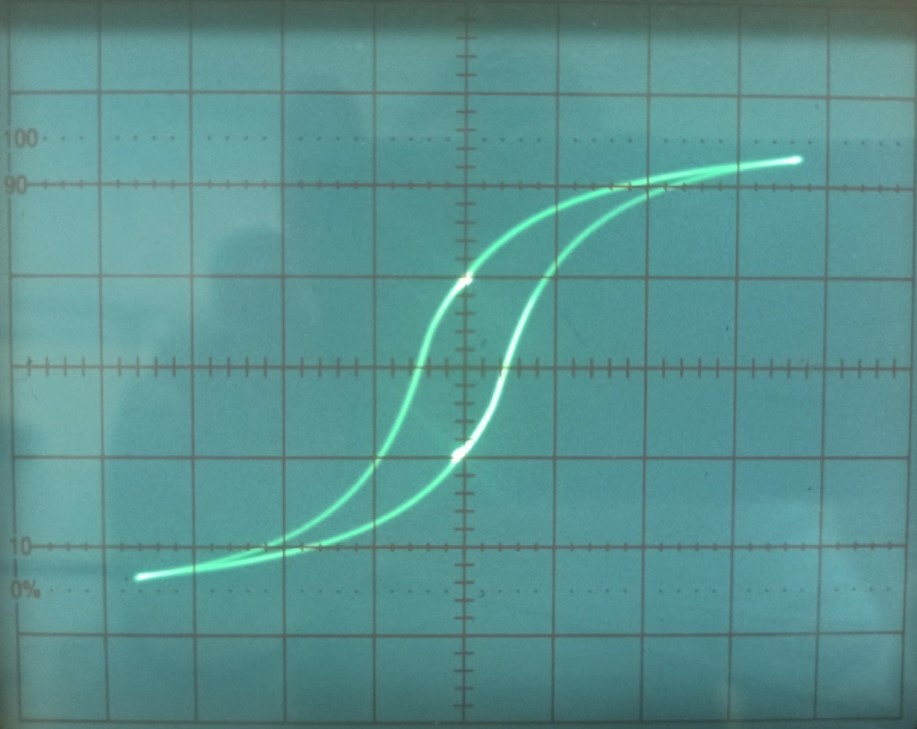
\includegraphics[scale=0.5]{PIC_4.jpg}
		\\\textbf{Рис. 4: } Предельная петля гистерезиса феррита
	\end{center}
	
	\begin{center}
		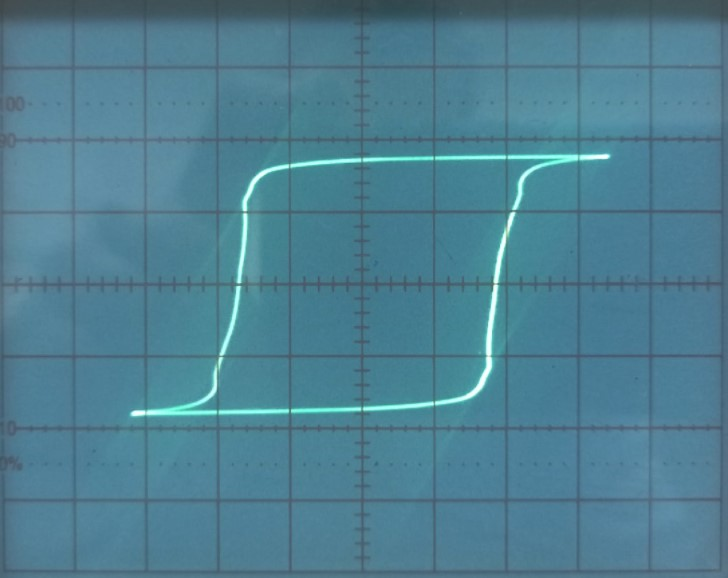
\includegraphics[scale=0.628]{PIC_5.jpg}
		\\\textbf{Рис. 5: } Предельная петля гистерезиса пермаллоя
	\end{center}
	
		\begin{center}
		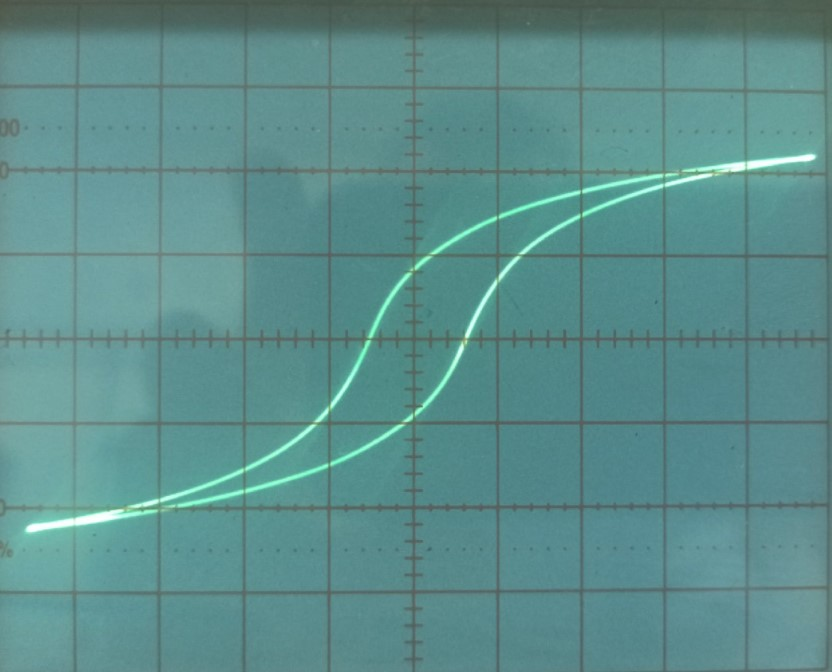
\includegraphics[scale=0.55]{PIC_6.jpg}
		\\\textbf{Рис. 6: } Предельная петля гистерезиса кремнистого железа
	\end{center}
	
В следующую таблицу занесём табличные данные для значений коэрцетивной силы $ H_c $ и индукции насыщения $ B_s $.

\paragraph{Проверка применимости теоретической выкладки} \hfill

Для этого рассчитаем $\tau$ -- постоянную времени $ RC $-цепочки. Для определения напряжений на входе и выходе интегрирующей ячейки соединим вход ячейки с обмоткой <<6,3 В>> трансформатора. Подключим Y-вход ЭО ко входу интегрирующей ячейки и отключим X-вход ЭО. Подберем такой ток, чтобы вертикальная прямая занимала большую часть экрана, и определим входное напряжение $U_{\text{вх}}=2y\cdot K_y=6,8\ \text{дел} \cdot 2\ \text{В/дел}=13,6\ \text{В}$. Не меняя тока, подключим Y-вход ЭО к выходу ячейки и аналогичным образом определим $U_{\text{вых}}=2y\cdot K_y=5,2\ \text{дел} \cdot 0,02\ \text{В/дел}=0,104\ \text{В}$. Рассчитаем $\tau=\frac{U_{\text{вх}}}{\omega U_{\text{вых}}}=\frac{13,6}{0,104\cdot2\pi\cdot 50}=0,416\ \text{c}$, где $\omega=2\pi\nu$. По определению $\tau_{RC}=R_\text{и}C_\text{и}=0,4\ \text{с}$. Так как $\tau\approx\tau_{RC}$, то условия применимости нашей теории выполнены.

\section{Выводы}
В ходе выполнения данной лабораторной работы были исследованы петли гистерезиса для трех различных образцов и получены характерные величины для каждого образца, приведем сравнительную таблицу:

\begin{center}
	\begin{tabular}{|c|c|c|c|c|}
		\hline
		Материал     & $H_c$, А/м & $\tilde{H_c}$, А/м  & $B_s$, Тл & $\tilde{B_s}$, Тл \\ \hline
		Феррит       & 7.27 $\pm$ 0.76     & 20      & 0.16 $\pm$ 0.01    & 0,27               \\ \hline
		Пермаллой    & 24.61 $\pm$ 2.20      & 11-40    & 1.58 $\pm$ 0.13  & 1.51               \\ \hline
		Крем. железо & 61.98 $\pm$ 7.30      & 50-100     & 0.88  $\pm$ 0.06    & 1.21               \\ \hline
	\end{tabular}
	\\\textbf{Табл. 5:} Сравнительная таблица
\end{center}
\end{document}